
\chapter{Resultat}

I detta kapitel redovisas kortfattat det resulterande läromaterialet. Även
resultaten från utvärderingen med testgruppen och mötena med Fäldt redovisas.

\begin{draft}

\section{Läromaterialet}
\label{sec:res_laromaterial}

Läromaterialet blev i slutändan en sammanvävning av domänspecifika språk som
modellerar fysik, och en lärotext som förklarar kopplingen mellan fysiken och de
domänspecifika språken. Figur~\ref{fig:smakprov_laromaterial} visar ett kort
utdrag ur läromaterialet. Där ses hur domänspecifika språk och lärotext
är sammanvävda. Ett längre utdrag finns i bilaga \ref{cha:utdrag}.

\begin{figure}[tph]
  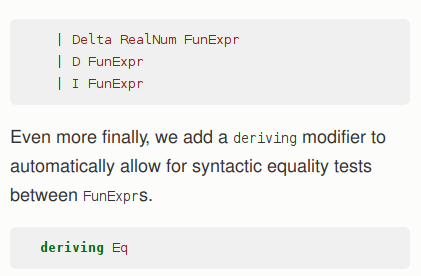
\includegraphics[width=\linewidth]{figure/smakprov_laromaterial.png}
  \caption{Ett smakprov över hur det resulterande läromaterialet ser ut.
           Lärotexten ligger mot den ljusgrå bakgrunden medan det
           domänspecifika språket ligger mot den
           mörkgrå.}~\label{fig:smakprov_laromaterial} 
\end{figure}

I läromaterialet finns även bilder och övningar.
Figur~\ref{fig:smakprov_bild_laromaterial} är ett exempel på en bild ur
läromaterialet. Notera speciellt den medvetet oseriösa ritningstekniken som är
tänkt att vara rolig och muntra upp läsaren. Övningar ligger både i den löpande
texten och i slutet av kapitlet. Övningarna i den löpande texten innebär oftast
att läsaren ska implementera en liten del av det aktuella domänspecifika språket
på egen hand. Det här illustreras i figur~\ref{fig:smakprov_ovning}.

\begin{figure}[tph]
    \centering
    \begin{subfigure}[t]{0.5\textwidth}
        \centering
        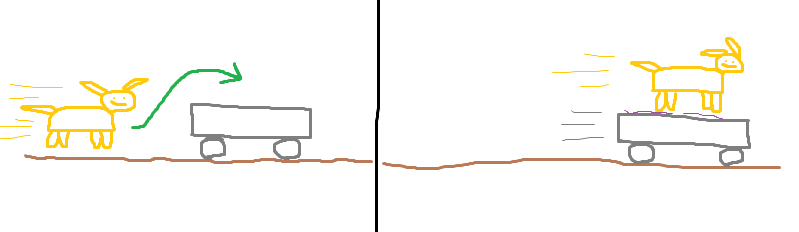
\includegraphics[width=0.9\linewidth]{figure/smakprov_bild_laromaterial.png}
        \caption{Exempel på en bild. Bilden visar hur en hund springer och
                 hoppar upp på en stillastående
                 vagn.}~\label{fig:smakprov_bild_laromaterial}
    \end{subfigure}% 
    ~~~
    \begin{subfigure}[t]{0.5\textwidth}
        \centering
        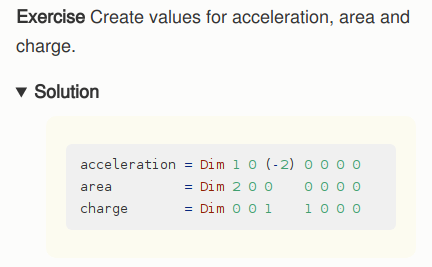
\includegraphics[width=0.9\linewidth]{figure/smakprov_ovning.png}
        \caption{Exempel på en övning. Övningen ligger som en del av den
                 löpande texten.}~\label{fig:smakprov_ovning}
    \end{subfigure}
    \caption{Exempel på en bild och en övning ur läromaterialet.} 
\end{figure}

Läromataterialet behandlar ett flertal områden inom fysik och matematik.
Fokuset är på klassisk mekanik samt till det området tillhörande matematik. I
sin fullständighet är de behandlade områdena:

\begin{itemize}
  \item Bevis
  \item Dimensioner
  \item Matematisk analys
  \item Vektorer
  \item Kompositioner och tillämpningar av ovanstående
\end{itemize}

I \textit{bevis}-kapitlet presenteras bevisföring med hjälp av Haskells
typsystem. Närmare bestämt används \textit{Curry Howard isomorfin}, som säger
att typer är påståenden och värden bevis.\cite{chi} Det exemplifieras genom att
kinematiska formler bevisas. 

\textit{Dimensioner} behandlar dimensioner, storheter och enheter inom fysiken.
Fysikaliska dimensioner införs på typnivå i Haskell för att visa likheten mellan
Haskells typsystem och hur man måste förhålla sig till dimensioner inom fysiken.
Typnivå-programmering\footnote{Vanligtvis manipuleras \textit{värden} när man
programmerar i Haskell och andra språk. Typnivå-programmering är precis som
vanlig programmering med skillnaden att den sker på typnivån, det vill säga,
typer modifieras. Läromaterialet~\cite{LYAP} hänvisas till för en utförligare
förklaring.} används för att göra likheterna så tydliga som möjligt.

I \textit{matematisk analys} konstrueras ett syntaxträd för algebraiska uttryck
och funktioner. Därefter implementeras symbolisk derivering och integrering på
syntaxträdet.

\textit{Vektorer} behandlar vektorer och vektoroperationer. Vektorer modelleras
som med hjälp av en typklass som dikterar vilka funktioner som varje
modell av en vektor måste implementera. Generall vektoroperationer såsom
addition och skalärprodukt implementerades sedan med hjälp av dessa funktioner
vilket skapade ett mycket generellt och lättanvänt gränssnitt. Quickcheck
användes för att verifiera lagarna som gäller för olika vektoroperationer,
vilket gav en generell säkerhet kring att implementationerna var korrekta.

I läromataterialet finns, förutom de fyra ovanstående grundläggande områdena,
även tillämpningar av dem på exempelproblem. Till exempel används dimensioner
till att lösa problem med fritt fall. De tillämpningar som behandlats är

\begin{itemize}
  \item Gundbräda
  \item Krafter på lådor
\end{itemize}

Gör PSSSO\footnote{På Samma Sätt Som Ovan} för de kompisita områdena, dvs skriv
vad varje handlar om.

\textit{Single particle mechanics} \textbf{TODO}

Läromaterialet blev publicerat på en hemsida\cite{LYAP} och all källkod finns
tillgänglig på projektets GitHub-repository.\cite{LYAP_repo} Texten är skriven
på engelska.

%\begin{binge}
%
%EXEMPEL PÅ ATT VI ANVÄNDER LITERAT STIL, OM DET SKULLE BEHÖVAS
%
%I Quantity så är detta tydligt. Då gjordes en `taste of types'' tidigt för att
%läsaren skulle förstå Quantity bättre, innan massa detaljer gicks %in på. Frågan
%är dock om detta ska gås in på i rapporten?
%
%\end{binge}

\section{Utvärderingen med testgruppen}~\label{sec:res_test}

Utfallet från utvärderingen med testgruppen var till övervägande del positivt.
Testgruppen tyckte läromaterialet var ett intressant och roligt sätt att
presentera fysik på. De tyckte att bilderna tjänade sitt syfte, att muntra upp
läsaren. 

En poäng som framfördes var att inte börja kapitlena för komplicerat. Istället
tyckte de att det skulle vara bra att börja enkelt, för att kunna hänga med i
både Haskell-koden och fysiken, för att därefter behandla ett område mer
detaljerat. Att visa ett kort exempel i Haskell för att sedan låta läsaren själv
göra något liknande var ett förslag på hur det kunde göras.

Utvärderingen var dock för kort för att det skulle framgå huruvida läsaren lärde
sig mest fysik eller mest Haskell. Det framgick heller inte om läromatarialet
uppmuntrade testgruppen att vilja lära sig mer fysik.

\section{Möten med Fäldt}~\label{sec:res_ake}

Åke Fäldt hade en överlag positiv syn på läromaterialet.\footnote{Det bör
påpekas att det som är återgivit här självklart har tolkats, och kan ha
missuppfattats, av projektgruppen. Fäldt ska med andra ord inte behöva stå till
svars för vad som står här.} Fäldt tyckte att det fanns flera saker
läromaterialet kunde bidra med. En bra sak var att läromaterialet ger att annat
perspektiv på fysiken, ett annat sätt att förklara den genom att göra det med
hjälp av domänspecifika språk.

En annan bra sak var den rigorösitet som domänspecifika språk leder till.
Eftersom de domänspecifika språken måste vara väldefinerade betyder det att alla
fysikalaiska koncept måste göras entydiga och även de blir väldefinerade.
Operationerna på dem kan enbart göras på det definerade sättet. Följden blir att
inget fusk kan göras i beräkningarna - alla steg måste vara fullständiga och
följa de regler som finns. Fäldt menade att det var en bra egenskap hos
läromaterialet, att detta rigorösa tankesätt och metodik som förmedlas hade
varit till nytta i problemlösning i fysikkursen.

Förutom ovanstående framgick även vilka områden i Fysik för ingenjörer som var
svåra för studenter. Detta finns redovisat i avsitt~\ref{sec:kontakt_faldt}

\end{draft}































